% Provenance (never printed): old terminale S material on absolute dating (the
% decay law recalled, the closed system, the rubidium-strontium isochron) and on
% the history of the age of the Earth (cooling, salt, sediments, then radioactivity,
% meteorites and 4.55 billion years). Owner (Sync 0/1): closed system, isochron,
% age of the Earth (as a defined notion). The decay law, the half-life and the
% dating equation are the physics books' (recalled); relative dating, absolute
% age, superposition, cross-cutting relationships and the eras are Book 1 g7's
% (recalled); the oldest zircons and the Acasta gneiss are g12.01's (quoted).
% Varden Hills granite 310 Ma and schist 480 Ma from figdata/shared/region.py;
% their isotope ratios are exercise data (figdata/grade-12/isochrons.py).
\chapter{Penanggalan Radiometrik dan Umur Bumi}\label{ch:g12:age-of-the-earth}

Pada tahun 1862 fisikawan William Thomson, yang kemudian menjadi Lord Kelvin,
menghitung \omterm{def:g12:age-of-the-earth:age}{umur Bumi} dari cara Bumi mendingin. Ia mengandaikan bahwa Bumi
terbentuk dalam keadaan lebur dan sejak itu terus kehilangan panasnya, lalu
bertanya berapa lama waktu yang diperlukan agar gradien suhu di dekat permukaan
turun sampai nilainya sekarang. Jawabannya adalah 96 juta tahun, di suatu
tempat antara 20 dan 400 juta tahun; pada tahun 1897 ia telah mempersempitnya
menjadi antara 20 dan 40 juta. Para ahli geologi menganggap waktu itu jauh
terlalu singkat untuk sejarah yang mereka baca di dalam batuan. Jawabannya
datang dari radioaktivitas, yang tidak dikenal Kelvin.
% ledger: holmes13:estimates, england:kelvin (Book 3 row)

\begin{omfigure}
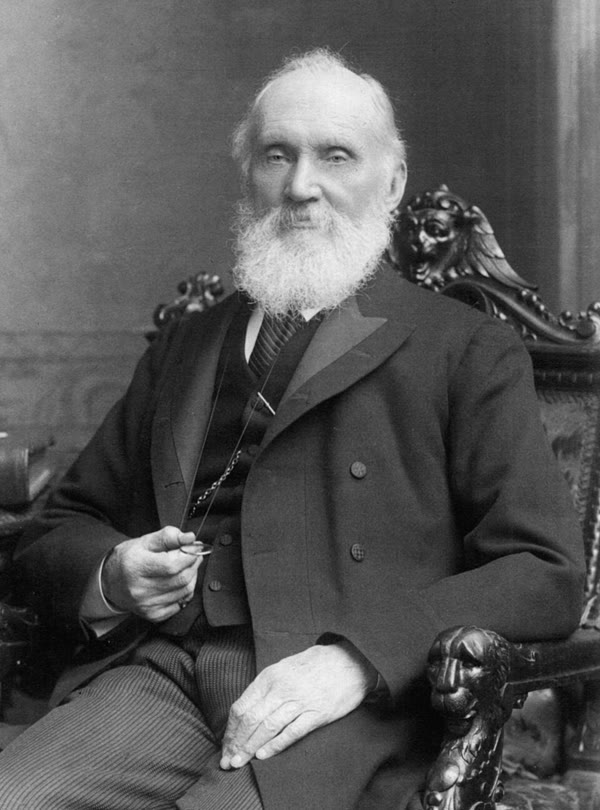
\includegraphics[height=5.2cm]{images/book2/g12-kelvin-1906.jpg}

{\small William Thomson, Lord Kelvin, pada tahun 1906. Foto Russell and Sons,
London (Smithsonian Institution Libraries, tidak diketahui adanya pembatasan hak
cipta).}
\end{omfigure}
% ledger: photo:g12-kelvin

\begin{recall}
Penanggalan relatif mengurutkan batuan dan peristiwa; umur absolut adalah
sebuah bilangan tahun (Buku 1, kelas 7). Sebuah isotop radioaktif, yaitu
induknya, meluruh secara acak menjadi isotop anak: jumlah $N$ atom induk yang
tersisa turun menurut $N = N_0\,e^{-\lambda t}$, dengan $\lambda$ konstanta
peluruhan, dan berkurang separuhnya setiap waktu paruh $T = \ln 2/\lambda$
(buku-buku fisika). Mineral tertua yang diketahui, zirkon dari Australia Barat,
berumur 4.4 miliar tahun (\cref{ch:g12:continental-crust}). Bumi juga
kehilangan panas yang terus dihasilkan oleh radioaktivitas, dan mantelnya
berkonveksi (\cref{ch:g12:internal-heat}).
\end{recall}
% ledger: wilde01:zircon

\section{Sejarah perkiraan}

Sebelum radioaktivitas, setiap perkiraan \omterm{def:g12:age-of-the-earth:age}{umur Bumi} bertumpu pada suatu proses
yang lajunya dianggap sudah diketahui.

\begin{center}
\small
\begin{tabular}{|p{0.19\linewidth}|p{0.42\linewidth}|p{0.25\linewidth}|}
\hline
siapa, kapan & metode dan apa yang diandaikannya & perkiraan \\
\hline
Phillips, 1860 & tebal lapisan sedimen dibagi laju pengendapan; mengandaikan laju yang tetap & 38 sampai 96 juta tahun \\
Kelvin, 1862 & pendinginan Bumi yang lebur hanya melalui konduksi, tanpa sumber panas di dalamnya & 20 sampai 400 juta tahun \\
G.\,H.~Darwin & waktu sejak Bulan terpisah dari Bumi, dari melambatnya gerak keduanya oleh pasang surut & setidaknya 56 juta tahun \\
Joly, 1899 & garam yang dibawa sungai ke laut, dibagi pasokan tahunannya; mengandaikan pasokan yang tetap dan tidak ada garam yang hilang & 80 sampai 100 juta tahun \\
\hline
\end{tabular}
\end{center}
% ledger: holmes13:estimates

\begin{history}[Panas yang terlewat oleh Kelvin]
Pada tahun 1903 Pierre Curie dan Albert Laborde menunjukkan bahwa radium
memancarkan panas, dan tak lama kemudian beberapa ilmuwan berpendapat bahwa panas
ini menjungkirbalikkan kesimpulan Kelvin. Setahun kemudian Ernest Rutherford,
yang berceramah dengan Kelvin di antara hadirin, mengingatkannya bahwa ia telah
membatasi \omterm{def:g12:age-of-the-earth:age}{umur Bumi} ``asalkan tidak ditemukan sumber panas baru''. Radioaktivitas
tampaknya merupakan sumber itu. Namun itu bukan kesalahan utama Kelvin: yang
paling memperpanjang pendinginan Bumi adalah \omterm{def:g12:internal-heat:convection}{konveksi mantel}, yang menjaga mantel
atas tetap panas dan gradien di dalam kerak tetap tinggi jauh lebih lama daripada
konduksi saja.
\end{history}
% ledger: england:kelvin (Book 3 row)

Radioaktivitas juga memberikan sebuah jam. Pada tahun 1907 Bertram Boltwood
menunjukkan bahwa mineral uranium yang seumur mengandung jumlah timbal yang
sama untuk setiap gram uranium: timbal itu dibuat oleh uranium. Pada tahun 1913
Arthur Holmes dapat menulis bahwa batuan tertua yang telah ditanggali berumur
\num{1600} juta tahun, dan pada tahun 1927 ia menempatkan \omterm{def:g12:age-of-the-earth:age}{umur Bumi} antara 1.6
dan 3.0 miliar tahun. Pada tahun 1956 Clair Patterson mengukur 4.55 miliar
tahun. Nilai saat ini adalah 4.54 miliar tahun, dengan ketelitian satu persen.
% ledger: holmes13:estimates, holmes27:age, patterson56:table, usgs:age-earth (Book 1 row)

\begin{omfigure}
\begin{tikzpicture}
\begin{axis}[omrecord, width=0.78\linewidth, height=6.2cm, ymode=log, xmin=1840, xmax=2040,
  ymin=1e7, ymax=2e10, xlabel={tahun perkiraan}, ylabel={perkiraan umur Bumi (tahun)},
  xtick={1850,1875,...,2025}, x tick label style={/pgf/number format/.cd, set thousands separator={}},
  ytick={1e7,1e8,1e9,1e10}, ymajorgrids=true, xmajorgrids=false]
% computed in figdata/grade-12/isochrons.py; ledger: holmes13:estimates, holmes27:age, patterson56:table, usgs:age-earth (Book 1 row)
\addplot[omDef, only marks, mark=*, mark size=1.8pt, error bars/.cd, y dir=both, y explicit]
  table[x=year, y=mid, y error minus expr=\thisrow{mid}-\thisrow{lo}, y error plus expr=\thisrow{hi}-\thisrow{mid}]
  {figdata/out/grade-12-isochrons-history.dat};
\addplot[omThm, densely dashed, domain=1840:2040, samples=2] {4.54e9};
\coordinate (k62) at (axis cs:1862,2.4e8);
\coordinate (k97) at (axis cs:1897,2.8e7);
\coordinate (jol) at (axis cs:1899,1e8);
\coordinate (h11) at (axis cs:1919,1.3e9);
\coordinate (pat) at (axis cs:1956,4.55e9);
\coordinate (now) at (axis cs:1845,4.54e9);
\end{axis}
\node[font=\scriptsize, anchor=west] at ([xshift=4pt]k62) {Kelvin 1862};
\node[font=\scriptsize, anchor=east] at ([xshift=-4pt]k97) {Kelvin 1897};
\node[font=\scriptsize, anchor=west] at ([xshift=4pt]jol) {Joly};
\node[font=\scriptsize, anchor=north] at (h11) {Holmes};
\node[font=\scriptsize, anchor=north west] at ([xshift=2pt, yshift=-3pt]pat) {Patterson};
\node[font=\scriptsize, text=omThm, anchor=south west] at (now) {kini, 4.54 miliar tahun};
\end{tikzpicture}

{\small Perkiraan \omterm{def:g12:age-of-the-earth:age}{umur Bumi} terhadap tahun dibuatnya perkiraan itu, pada skala
logaritmik; batang-batang meliputi rentang yang diberikan setiap penulis. Titik
Holmes tahun 1913 adalah umur batuan tertua yang telah ditanggali pada waktu
itu, sebuah batas bawah. Sumber: Holmes (1913, 1927); Patterson (1956); U.S.
Geological Survey.}
\end{omfigure}

\section{Sebuah jam radioaktif}

Jam radioaktif hanya bekerja bila tidak ada yang ditambahkan ke dalamnya atau
diambil darinya sejak jam itu mulai berjalan.

\begin{definition}[Sistem tertutup]\label{def:g12:age-of-the-earth:closed-system}
Yang disebut \emph{sistem tertutup}\index{sistem tertutup} untuk sebuah isotop
induk dan anaknya adalah batuan atau mineral yang, sejak saat jamnya mulai
berjalan, tidak dimasuki atau ditinggalkan satu atom pun dari induk atau anak
itu, selain melalui peluruhan induk menjadi anak.
\end{definition}
% ledger: tulane:radiometric

Untuk sebuah mineral, jam itu mulai berjalan ketika mineral itu mengkristal dari
magma, atau lebih tepatnya ketika mineral itu telah cukup dingin sehingga atom-atom
berhenti keluar masuk. Pemanasan, fluida panas,
atau pelapukan dapat membuka sistem itu kembali, dan umur yang kemudian diukur
menjadi salah, atau menanggali peristiwa yang kemudian itu.
% ledger: tulane:radiometric

Menghitung atom anak dalam sebuah \omterm{def:g12:age-of-the-earth:closed-system}{sistem tertutup} memberikan umurnya, asalkan
kita tahu berapa banyak yang ada pada awalnya. Biasanya kita tidak tahu.
Rubidium-87 meluruh menjadi stronsium-87, tetapi setiap mineral juga menyerap
sejumlah stronsium-87 ketika terbentuk. Metode \omterm{def:g12:age-of-the-earth:isochron}{isokron} mengatasi hal ini dengan
mengukur beberapa mineral dari satu batuan.

\section{Isokron}

Stronsium mempunyai sebuah isotop, stronsium-86, yang stabil dan tidak dihasilkan
oleh peluruhan apa pun: dalam \omterm{def:g12:age-of-the-earth:closed-system}{sistem tertutup} jumlahnya tetap sama, dan isotop
itu berfungsi sebagai tolok ukur. Rasio isotop $^{87}\mathrm{Sr}/^{86}\mathrm{Sr}$ dan
$^{87}\mathrm{Rb}/^{86}\mathrm{Sr}$ adalah besaran yang diukur oleh spektrometer massa.

\begin{theorem}[Persamaan isokron]\label{thm:g12:age-of-the-earth:isochron}
Dalam sebuah mineral yang telah menjadi \omterm{def:g12:age-of-the-earth:closed-system}{sistem tertutup} selama waktu $t$,
\[
  \left(\frac{^{87}\mathrm{Sr}}{^{86}\mathrm{Sr}}\right)_{\text{kini}}
  = \left(\frac{^{87}\mathrm{Sr}}{^{86}\mathrm{Sr}}\right)_{0}
  + \left(\frac{^{87}\mathrm{Rb}}{^{86}\mathrm{Sr}}\right)_{\text{kini}}
  \left(e^{\lambda t} - 1\right),
\]
dengan indeks 0 menandai nilai ketika jam itu mulai berjalan dan $\lambda$
konstanta peluruhan rubidium-87.
\end{theorem}

\begin{proof}
Misalkan $P$ jumlah atom rubidium-87 sekarang dan $P_0$ ketika jam itu mulai
berjalan. Menurut hukum peluruhan $P = P_0\,e^{-\lambda t}$, sehingga $P_0 = P\,e^{\lambda t}$,
dan jumlah atom yang telah meluruh adalah $P_0 - P = P\,(e^{\lambda t}-1)$.
Dalam \omterm{def:g12:age-of-the-earth:closed-system}{sistem tertutup} setiap atom itu telah menjadi satu atom stronsium-87, yang
ditambahkan pada $D_0$ atom yang ada pada awalnya: $D = D_0 + P\,(e^{\lambda
t}-1)$. Membaginya dengan jumlah atom stronsium-86, yang tidak berubah,
memberikan persamaan itu.
\end{proof}
% ledger: tulane:radiometric

Mineral-mineral sebuah granit mengkristal dari satu magma, sehingga semuanya
bermula dengan rasio $(^{87}\mathrm{Sr}/^{86}\mathrm{Sr})_0$ yang sama. Tetapi
mineral-mineral itu menyerap rubidium dalam jumlah yang sangat berbeda. Semuanya
mempunyai $t$ yang sama dan rasio awal yang sama, sehingga persamaan itu
menyatakan bahwa titik-titiknya terletak pada satu garis lurus.

\begin{definition}[Isokron]\label{def:g12:age-of-the-earth:isochron}
Yang disebut \emph{isokron}\index{isokron} adalah garis lurus tempat terletaknya
titik-titik mineral atau batuan yang terbentuk pada waktu yang sama dari sumber
yang sama dan sejak itu tetap menjadi \omterm{def:g12:age-of-the-earth:closed-system}{sistem tertutup}, bila rasio isotop anak
terhadap isotop stabil diplot terhadap rasio isotop induk terhadap isotop
stabil. Kemiringannya memberikan umurnya, dan titik tempat garis itu memotong
sumbu tegak memberikan rasio awalnya.
\end{definition}
% ledger: tulane:radiometric

\begin{proposition}[Umur dari kemiringan]\label{prop:g12:age-of-the-earth:slope}
Bila sebuah \omterm{def:g12:age-of-the-earth:isochron}{isokron} mempunyai kemiringan $m$, umurnya adalah
\[
  t = \frac{\ln(1+m)}{\lambda}.
\]
\end{proposition}

\begin{proof}
Dengan membandingkannya dengan persamaan \omterm{def:g12:age-of-the-earth:isochron}{isokron}, $m = e^{\lambda t} - 1$, sehingga
$e^{\lambda t} = 1 + m$, $\lambda t = \ln(1+m)$, dan $t = \ln(1+m)/\lambda$.
\end{proof}

Untuk rubidium-87, $\lambda = \num{1.3972e-11}$ per tahun, yaitu waktu paruh
$\ln 2/\lambda \approx 49.6$ miliar tahun: lebih dari sepuluh kali \omterm{def:g12:age-of-the-earth:age}{umur
Bumi}.
% ledger: villa22:rb87

\begin{method}[Menanggali batuan dengan isokron]\label{met:g12:age-of-the-earth:isochron}
\begin{enumerate}
  \item Pisahkan beberapa mineral dari batuan itu (atau ambillah beberapa
        sampelnya) yang jumlah rubidiumnya berbeda-beda.
  \item Ukurlah pada masing-masing rasio $^{87}\mathrm{Rb}/^{86}\mathrm{Sr}$ ($x$)
        dan $^{87}\mathrm{Sr}/^{86}\mathrm{Sr}$ ($y$).
  \item Plotkan $y$ terhadap $x$ dan periksalah bahwa titik-titiknya terletak
        pada satu garis lurus: bila ada yang tidak, sampel itu bukan \omterm{def:g12:age-of-the-earth:closed-system}{sistem tertutup}.
  \item Ambillah kemiringan $m$ garis itu, lalu hitung $t = \ln(1+m)/\lambda$.
  \item Bacalah rasio awalnya di tempat garis itu memotong sumbu tegak.
\end{enumerate}
\end{method}

\begin{example}[Granit Varden]\label{ex:g12:age-of-the-earth:varden}
Granit Perbukitan Varden, wilayah rekaan seri ini, memberikan rasio-rasio
berikut (data latihan):
\begin{center}
\small
\begin{tabular}{|l|c|c|}
\hline
sampel & $^{87}\mathrm{Rb}/^{86}\mathrm{Sr}$ & $^{87}\mathrm{Sr}/^{86}\mathrm{Sr}$ \\
\hline
plagioklas & 0.35 & 0.70952 \\
hornblende  & 1.20 & 0.71321 \\
batuan utuh  & 3.10 & 0.72146 \\
feldspar-K  & 6.40 & 0.73578 \\
biotit     & 24.0 & 0.81218 \\
\hline
\end{tabular}
\end{center}
Melalui plagioklas dan biotit, kemiringannya
$m = (0.81218 - 0.70952)/(24.0 - 0.35) \approx 0.004341$. Maka
$t = \ln(1.004341)/\num{1.3972e-11} \approx \num{3.10e8}$ tahun:
granit itu berumur 310 juta tahun. Garis itu memotong sumbu tegak pada
$0.70952 - 0.35 \times 0.004341 \approx 0.7080$, yaitu rasio awalnya.
\end{example}
% values: granite_age_Ma 310.0, granite_intercept 0.70800 (isochrons.py)

\begin{omfigure}
\begin{tikzpicture}
\begin{axis}[omrecord, width=0.7\linewidth, height=6cm, xmin=0, xmax=26, ymin=0.695, ymax=0.82, ytick={0.70,0.72,...,0.82},
  xlabel={$^{87}\mathrm{Rb}/^{86}\mathrm{Sr}$}, ylabel={$^{87}\mathrm{Sr}/^{86}\mathrm{Sr}$},
  y tick label style={/pgf/number format/.cd, fixed, fixed zerofill, precision=2}]
% computed in figdata/grade-12/isochrons.py (exercise data, Varden granite 310 Ma); ledger: villa22:rb87
\addplot[omDef, line width=0.9pt] table[x=x, y=y] {figdata/out/grade-12-isochrons-graniteln.dat};
\addplot[omThm, only marks, mark=*, mark size=2pt] table[x=rbsr, y=srsr] {figdata/out/grade-12-isochrons-granite.dat};
\addplot[black!60, densely dotted, domain=0:26, samples=2] {0.7080};
\coordinate (pl) at (axis cs:0.35,0.70952);
\coordinate (hb) at (axis cs:1.2,0.71321);
\coordinate (wr) at (axis cs:3.1,0.72146);
\coordinate (kf) at (axis cs:6.4,0.73578);
\coordinate (bt) at (axis cs:24,0.81218);
\coordinate (sl) at (axis cs:12,0.762);
\coordinate (in) at (axis cs:9,0.7082);
\coordinate (plhb) at (axis cs:0.6,0.737);
\coordinate (plhbpt) at (axis cs:0.9,0.7125);
\end{axis}
\node[font=\scriptsize, anchor=north west] at ([xshift=1pt]wr) {batuan utuh};
\node[font=\scriptsize, anchor=north west] at ([xshift=1pt]kf) {feldspar-K};
\node[font=\scriptsize, anchor=east] at ([xshift=-3pt]bt) {biotit};
\node[font=\scriptsize, anchor=south west, align=left, inner sep=1pt] (plhblab) at (plhb) {plagioklas,\\hornblende};
\draw[black!60, line width=0.4pt] (plhblab.south) -- (plhbpt);
\node[font=\scriptsize, text=omDef, anchor=south east] at (sl) {\shortstack[r]{kemiringan $0.004341$:\\310 juta tahun}};
\node[font=\scriptsize, text=black!70, anchor=south west] at (in) {rasio awal 0.7080 (waktu 0)};
\end{tikzpicture}

{\small \omterm{def:g12:age-of-the-earth:isochron}{Isokron} rubidium--stronsium granit Varden (data latihan). Ketika granit
itu terbentuk, semua mineralnya terletak pada garis mendatar yang
bertitik-titik; sejak itu masing-masing telah naik sebanding dengan
rubidiumnya, dan kini semuanya terletak pada garis yang utuh.}
\end{omfigure}

\begin{inthelab}[Menimbang atom]
Rasio-rasio itu diukur dengan spektrometer massa. Beberapa miligram mineral
dilarutkan dalam asam, dan stronsium dipisahkan dari rubidium secara kimia,
karena kalau tidak, kedua isotop bermassa 87 itu akan terhitung bersama.
Stronsium itu, yang diletakkan pada sebuah filamen logam dan dipanaskan dalam
vakum, melepaskan ion; sebuah medan listrik mempercepatnya dan sebuah magnet
membelokkan lintasannya, ion yang lebih ringan lebih kuat daripada yang lebih
berat, sehingga setiap isotop sampai di kolektornya sendiri. Arus-arusnya
memberikan rasio-rasio itu.
\end{inthelab}

\begin{omfigure}
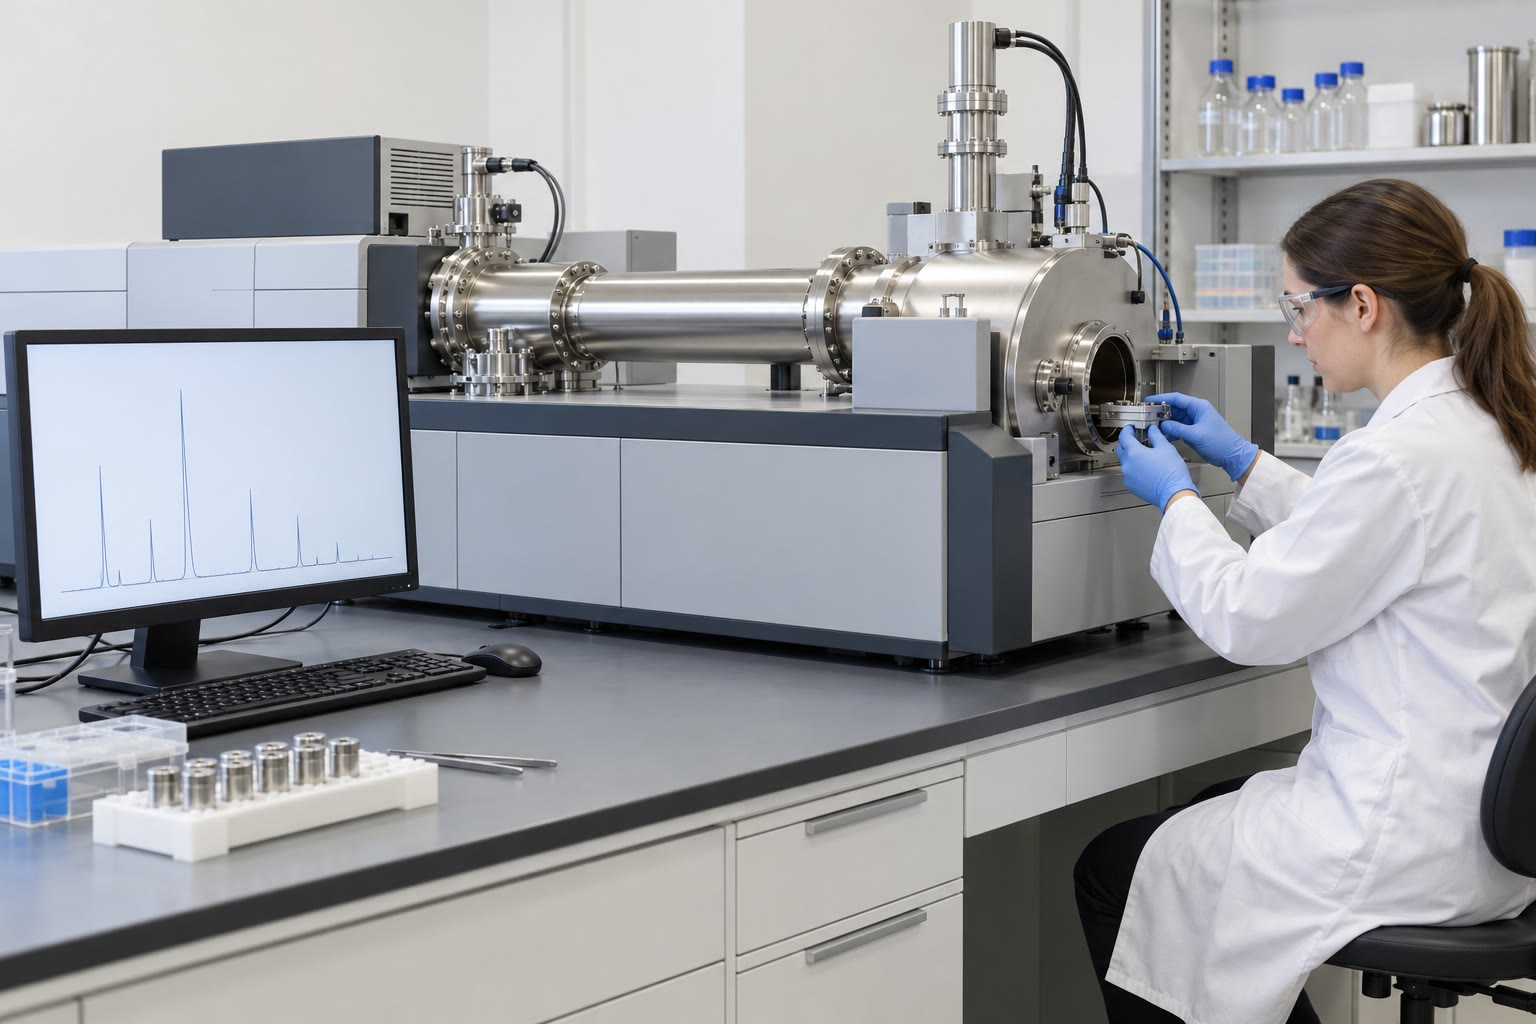
\includegraphics[width=0.66\linewidth]{images/book2/ai/g12-mass-spectrometer-lab.jpg}

{\small Sebuah spektrometer massa di laboratorium: sebuah sampel sedang
dimasukkan di ujung sumbernya (ilustrasi AI).}
\end{omfigure}

Rasio awal itu juga merupakan petunjuk tentang asal magma. Rubidium lebih
menyukai lelehan ketika mantel meleleh, sehingga dari zaman ke zaman rubidium
terpusat di dalam \omterm{def:g12:continental-crust:continental-crust}{kerak benua}, yang karena itu telah membuat lebih banyak
stronsium-87: batuan kerak mempunyai $^{87}\mathrm{Sr}/^{86}\mathrm{Sr}$ yang
lebih tinggi daripada batuan mantel. Magma dari kerak yang meleleh mewarisi
rasio yang tinggi itu.
% ledger: tulane:radiometric

\section{Umur Bumi}

Tidak ada batuan di Bumi yang berasal dari awal Bumi: batuan tertua yang
diketahui, gneis Acasta, berumur 4.03 miliar tahun, dan zirkon tertua 4.4
miliar. Sejak itu permukaannya telah dileburkan, dikikis, dan didaur ulang.
Penanggalan Bumi itu sendiri berasal dari meteorit, pecahan-pecahan benda kecil
yang terbentuk bersama planet-planet dan sebagian di antaranya tetap menjadi
\omterm{def:g12:age-of-the-earth:closed-system}{sistem tertutup} sejak saat itu.
% ledger: bowring99:acasta, wilde01:zircon, usgs:age-earth (Book 1 row)

\begin{definition}[Umur Bumi]\label{def:g12:age-of-the-earth:age}
Yang disebut \emph{umur Bumi}\index{umur Bumi} adalah waktu sejak Bumi terbentuk
melalui akresi benda-benda yang lebih kecil, pada saat lahirnya Tata Surya.
Diukur dari meteorit dengan penanggalan radiometrik, umur itu adalah
\num{4.54} miliar tahun, dengan ketelitian satu persen.
\end{definition}
% ledger: usgs:age-earth (Book 1 row)

Pada tahun 1956 Clair Patterson mengukur isotop-isotop timbal dalam tiga
meteorit batu dan dua meteorit besi. Dua isotop timbal dihasilkan oleh
peluruhan uranium, timbal-206 dari uranium-238 dan timbal-207 dari uranium-235,
sedangkan timbal-204 tidak dihasilkan oleh peluruhan apa pun. Seperti pada
stronsium, titik-titik meteorit yang terbentuk pada waktu yang sama terletak
pada satu garis lurus, bila
$^{207}\mathrm{Pb}/^{204}\mathrm{Pb}$ diplot terhadap
$^{206}\mathrm{Pb}/^{204}\mathrm{Pb}$. Meteorit besi Canyon Diablo, di
Arizona, hampir tidak mengandung uranium: timbalnya tidak berubah sejak meteorit
itu terbentuk, dan menandai ujung bawah garis itu, yaitu timbal yang dimiliki
Tata Surya pada awalnya.
% ledger: patterson56:table, patterson56:constants, usgs:age-earth (Book 1 row: Canyon Diablo troilite)

\begin{omfigure}
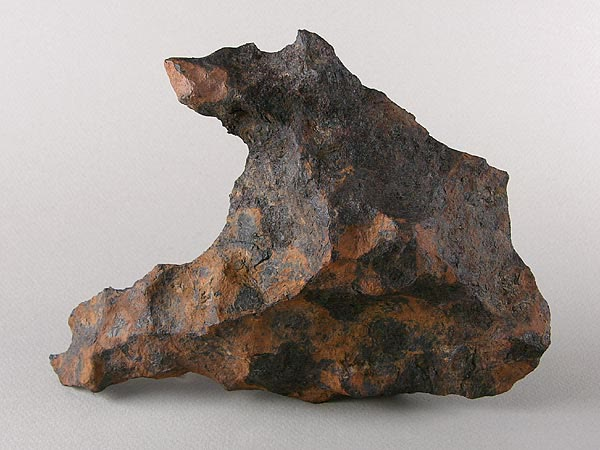
\includegraphics[height=4.2cm]{images/book2/g12-canyon-diablo-meteorite.jpg}

{\small Sebuah pecahan meteorit besi Canyon Diablo, \qty{2641}{g}.
Foto Geoffrey Notkin, CC~BY-SA~2.5 (Wikimedia Commons).}
\end{omfigure}
% ledger: photo:g12-canyon-diablo

Untuk timbal, kemiringan $m$ bergantung pada umur melalui kedua isotop uranium;
hubungan itu di sini diterima tanpa bukti. Dengan konstanta yang dipakai Patterson,
\[
  m = \frac{1}{137.8}\,\frac{e^{\lambda_{235}t}-1}{e^{\lambda_{238}t}-1},
  \qquad \lambda_{235} = \num{9.72e-10},\ \lambda_{238} = \num{1.537e-10}
  \text{ per tahun},
\]
yang memberikan:
\begin{center}
\small
\begin{tabular}{|l|c|c|c|c|c|c|}
\hline
umur (miliar tahun) & 4.40 & 4.45 & 4.50 & 4.55 & 4.60 & 4.65 \\
kemiringan $m$ & 0.533 & 0.551 & 0.570 & 0.590 & 0.610 & 0.632 \\
\hline
\end{tabular}
\end{center}
% ledger: patterson56:constants
% values: pb_slope at 4.40-4.65 Ga (isochrons.py pb_slope)

\begin{omfigure}
\begin{tikzpicture}
\begin{axis}[omrecord, width=0.72\linewidth, height=6cm, xmin=0, xmax=56, ymin=0, ymax=40,
  xlabel={$^{206}\mathrm{Pb}/^{204}\mathrm{Pb}$}, ylabel={$^{207}\mathrm{Pb}/^{204}\mathrm{Pb}$}]
% computed in figdata/grade-12/isochrons.py; ledger: patterson56:table
\addplot[omDef, line width=0.9pt] table[x=x, y=y] {figdata/out/grade-12-isochrons-pbln.dat};
\addplot[omThm, only marks, mark=*, mark size=2pt] table[x=r206, y=r207, restrict expr to domain={\thisrow{idx}}{1:5}] {figdata/out/grade-12-isochrons-pbpb.dat};
\addplot[black, only marks, mark=o, mark size=2.6pt, line width=0.8pt] table[x=r206, y=r207, restrict expr to domain={\thisrow{idx}}{6:6}] {figdata/out/grade-12-isochrons-pbpb.dat};
\coordinate (nl) at (axis cs:50.28,34.86);
\coordinate (fc) at (axis cs:19.48,15.76);
\coordinate (cd) at (axis cs:9.5,10.36);
\coordinate (sed) at (axis cs:19.0,15.5);
\coordinate (sl) at (axis cs:30,25);
\end{axis}
\node[font=\scriptsize, anchor=north west] at ([xshift=2pt]nl) {Nuevo Laredo};
\node[font=\scriptsize, anchor=north west, align=left] at ([xshift=4pt, yshift=-2pt]fc) {Forest City, Modoc;\\sedimen samudra (lingkaran)};
\node[font=\scriptsize, anchor=north west, align=left] at ([xshift=3pt, yshift=-3pt]cd) {Canyon Diablo, Henbury (besi)};
\node[font=\scriptsize, text=omDef, anchor=south east] at (sl) {\shortstack[r]{kemiringan 0.603:\\sekitar 4.6 miliar tahun}};
\end{tikzpicture}

{\small \omterm{def:g12:age-of-the-earth:isochron}{Isokron} timbal Patterson: kelima meteorit terletak pada satu garis,
demikian pula, hampir, timbal dari sebuah sedimen samudra modern, yang mewakili
Bumi. Sumber: Patterson (1956), Tabel~1.}
\end{omfigure}
% values: pb_slope 0.6026, pb_age_Ga 4.58, sediment_residual -0.39 (isochrons.py)

Garis yang ditarik melalui kelima titik itu mempunyai kemiringan sekitar 0.603,
di antara kemiringan untuk 4.55 dan 4.60 miliar tahun pada tabel. Hasil
Patterson sendiri, dengan memperhitungkan galat pengukuran dan galat konstanta
peluruhan, adalah 4.55 miliar tahun, plus minus 0.07. Ia kemudian mengukur
timbal dari sebuah sedimen samudra modern, yang mencampur timbal dari sebagian
besar massa kerak Bumi: titiknya terletak pada garis yang sama. Timbal Bumi
telah berevolusi seperti timbal meteorit, selama waktu yang sama: Bumi seumur
dengan meteorit-meteorit itu.
% ledger: patterson56:table

Sejak itu, ratusan pengukuran telah menegaskannya. Meteorit memberikan umur
dari 4.53 sampai 4.58 miliar tahun, dan zat padat tertua di Tata Surya,
inklusi-inklusi kecil yang kaya kalsium dan aluminium yang dijumpai di dalam
sebagian meteorit, terbentuk \num{4567.30} juta tahun yang lalu, plus minus
0.16. Bumi terbentuk kemudian dari bahan seperti itu, itulah sebabnya umurnya,
4.54 miliar tahun, sedikit lebih kecil daripada umur bahan itu.
% ledger: usgs:age-earth (Book 1 row), connelly12:cai

\section{Latihan}

\begin{exercise}[$\star$]\label{exo:g12:age-of-the-earth:1}
Sebutkan istilahnya: (a) mineral yang tidak dimasuki atau ditinggalkan satu
atom induk atau anak pun sejak jamnya mulai berjalan; (b) garis lurus tempat
terplotnya mineral-mineral yang seumur dan sesumber; (c) waktu sejak Bumi
terbentuk melalui akresi.
\end{exercise}

\begin{exercise}[$\star$]\label{exo:g12:age-of-the-earth:2}
Dengan tabel granit Varden, urutkan kelima sampelnya menurut rasio rubidium-87
terhadap stronsium-86, mulai dari yang terendah. Manakah yang terplot paling
tinggi pada \omterm{def:g12:age-of-the-earth:isochron}{isokron}, dan mengapa sampel itu telah membuat stronsium-87 paling
banyak?
\end{exercise}

\begin{exercise}[$\star$]\label{exo:g12:age-of-the-earth:3}
Hitung waktu paruh rubidium-87 dari konstanta peluruhannya,
\num{1.3972e-11} per tahun. Berapa kali \omterm{def:g12:age-of-the-earth:age}{umur Bumi} waktu paruh itu?
\end{exercise}

\begin{exercise}[$\star$]\label{exo:g12:age-of-the-earth:4}
Hitung $e^{\lambda t} - 1$ untuk rubidium-87 untuk $t = 310$ juta tahun dan
$t = 480$ juta tahun.
\end{exercise}

\begin{exercise}[$\star$]\label{exo:g12:age-of-the-earth:5}
Urutkan menurut tanggalnya perkiraan Phillips, Holmes (1927), Joly, Kelvin
(1862), dan Patterson. Berapa kali lebih besar \omterm{def:g12:age-of-the-earth:age}{umur Bumi} saat ini daripada
batas atas perkiraan Joly?
\end{exercise}

\begin{exercise}[$\star\star$]\label{exo:g12:age-of-the-earth:6}
Sebuah mineral granit Varden (310 juta tahun, rasio awal 0.7080)
mempunyai $^{87}\mathrm{Rb}/^{86}\mathrm{Sr} = 10.0$. Berapa
$^{87}\mathrm{Sr}/^{86}\mathrm{Sr}$-nya sekarang? Berapa nilainya ketika
granit itu terbentuk?
\end{exercise}

\begin{exercise}[$\star\star$]\label{exo:g12:age-of-the-earth:7}
Empat sampel sekis Varden memberikan $(x, y)$ = (0.90, 0.71806),
(2.60, 0.72950), (5.10, 0.74632), dan (9.40, 0.77525), dengan $x =
{}^{87}\mathrm{Rb}/^{86}\mathrm{Sr}$ dan $y = {}^{87}\mathrm{Sr}/^{86}\mathrm{Sr}$.
(1) Dari sampel pertama dan terakhir, hitung kemiringan dan umurnya.
(2) Periksalah bahwa kedua sampel tengah terletak pada garis yang sama.
(3) Apakah hasilnya sesuai dengan 310 juta tahun granit itu dan prinsip
hubungan potong-memotong?
\end{exercise}

\begin{exercise}[$\star\star$]\label{exo:g12:age-of-the-earth:8}
Mengapa batuan yang semua mineralnya mempunyai rasio rubidium terhadap
stronsium yang sama tidak memberikan \omterm{def:g12:age-of-the-earth:isochron}{isokron}? Mengapa biotit, dalam granit
Varden, menetapkan kemiringan lebih baik daripada mineral-mineral lainnya?
\end{exercise}

\begin{exercise}[$\star\star$]\label{exo:g12:age-of-the-earth:9}
Lama setelah granit Varden terbentuk, sebuah fluida panas membuat biotitnya
kehilangan sebagian stronsium-87-nya. (1) Ke mana titiknya berpindah pada
diagram \omterm{def:g12:age-of-the-earth:isochron}{isokron}? (2) Umur berapa yang kemudian diberikan oleh biotit dan
plagioklas saja: terlalu tua atau terlalu muda? (3) Bagaimana metode \omterm{def:g12:age-of-the-earth:isochron}{isokron}
mengungkapkan masalah itu?
\end{exercise}

\begin{exercise}[$\star\star$]\label{exo:g12:age-of-the-earth:10}
(1) Berapa kali lebih lama \omterm{def:g12:age-of-the-earth:age}{umur Bumi} daripada 96 juta tahun Kelvin? (2) Joly
mengandaikan bahwa sungai membawa garam ke laut dengan laju yang tetap dan
bahwa tidak ada garam yang meninggalkan laut. Andaian mana yang, bila salah,
membuat umurnya terlalu singkat, dan mengapa?
\end{exercise}

\begin{exercise}[$\star\star$]\label{exo:g12:age-of-the-earth:11}
Dengan nilai-nilai Patterson untuk Canyon Diablo (9.46, 10.34) dan Nuevo Laredo
(50.28, 34.86), hitung kemiringan garis yang melalui kedua meteorit itu, lalu
bacalah umurnya dari tabel kemiringan.
\end{exercise}

\begin{exercise}[$\star\star\star$]\label{exo:g12:age-of-the-earth:12}
Sebuah basalt di wilayah Varden, yang juga berumur 310 juta tahun, mempunyai
rasio awal 0.7035, dibandingkan dengan 0.7080 untuk granit. (1) Batuan mana
yang lebih mungkin berasal dari mantel yang meleleh, dan mana yang dari kerak
yang meleleh? (2) Jelaskan alasannya dengan apa yang kamu ketahui tentang
rubidium. (3) Mungkinkah keduanya mengkristal dari satu magma?
\end{exercise}

\begin{exercise}[$\star\star\star$]\label{exo:g12:age-of-the-earth:13}
(1) Berapa bagian rubidium-87 yang ada ketika Bumi terbentuk masih tersisa
sekarang? Dan berapa bagian uranium-238 (waktu paruh 4.47 miliar tahun)?
(2) Berapa kemiringan \omterm{def:g12:age-of-the-earth:isochron}{isokron} rubidium--stronsium untuk batuan yang berumur
sejuta tahun? Mengapa rubidium--stronsium merupakan jam yang buruk untuk batuan
muda?
\end{exercise}

\begin{exercise}[$\star\star\star$]\label{exo:g12:age-of-the-earth:14}
Garis yang melalui kelima meteorit Patterson adalah $y = 4.438 + 0.6026\,x$.
(1) Berapa $^{207}\mathrm{Pb}/^{204}\mathrm{Pb}$ yang diramalkannya untuk
sedimen samudra, pada $x = 19.0$? Patterson mengukur 15.5: berapa persen
selisih keduanya? (2) Umur berapa yang diberikan kemiringan 0.6026, menurut
tabel? Bandingkan dengan $4.55 \pm 0.07$ miliar tahun Patterson.
\end{exercise}

\begin{exercise}[$\star\star\star$]\label{exo:g12:age-of-the-earth:15}
Kelvin mengandaikan bahwa seluruh panas yang hilang dari Bumi, \qty{46.7}{TW}
saat ini, adalah panas simpanan. (1) Radioaktivitas menggantikan sekitar
\qty{24.4}{TW} di antaranya. Berapa kali hal itu, dengan sendirinya,
memperpanjang waktu untuk kehilangan sejumlah simpanan panas tertentu?
(2) Bermula dari 96 juta tahun, apakah ini cukup untuk mencapai umur yang
sebenarnya? (3) Apa yang terlewat oleh Kelvin yang lebih penting?
\end{exercise}

\begin{problem}[{Soal akhir pekan --- Menanggali granit Varden}]
\label{pb:g12:age-of-the-earth:1}
% exercise data from figdata/grade-12/isochrons.py; ledger: villa22:rb87, tulane:radiometric, ics:base.Carboniferous, ics:base.Permian
Granit Perbukitan Varden, wilayah rekaan seri ini, memotong sekis di
sekitarnya. Sebuah laboratorium mengukur lima sampelnya (contoh di atas):
plagioklas (0.35, 0.70952), hornblende (1.20, 0.71321), batuan utuh (3.10,
0.72146), feldspar-K (6.40, 0.73578), dan biotit (24.0, 0.81218), masing-masing
sebagai
$(^{87}\mathrm{Rb}/^{86}\mathrm{Sr},\ ^{87}\mathrm{Sr}/^{86}\mathrm{Sr})$.
Konstanta peluruhan rubidium-87 adalah \num{1.3972e-11} per tahun.

\medskip
\noindent\textbf{Bagian I --- Sampel-sampelnya.}
\begin{enumerate}
  \item Sampel mana yang paling kaya rubidium dibandingkan dengan stronsium?
  \item Mengapa semua mineral itu bermula dengan
        $^{87}\mathrm{Sr}/^{86}\mathrm{Sr}$ yang sama?
  \item Mengapa rasio-rasio itu diambil terhadap stronsium-86?
  \item Isotop mana dari ketiga isotop itu yang telah bertambah sejak granit
        itu terbentuk, dan mengapa?
  \item Seperti apa kelima titik itu pada diagram ketika granit itu baru saja
        terbentuk?
\end{enumerate}

\medskip
\noindent\textbf{Bagian II --- Garis isokron.}
\begin{enumerate}[resume]
  \item Hitung kemiringan melalui plagioklas dan biotit.
  \item Hitung kemiringan melalui plagioklas dan batuan utuh.
  \item Bandingkan kedua kemiringan itu. Mana yang lebih dapat diandalkan, dan
        mengapa?
  \item Carilah tempat garis dari pertanyaan 6 memotong sumbu tegak.
  \item Periksalah bahwa feldspar-K terletak pada garis itu.
\end{enumerate}

\medskip
\noindent\textbf{Bagian III --- Kemiringan dan umur.}
\begin{enumerate}[resume]
  \item Tuliskan hubungan antara kemiringan dan $e^{\lambda t}$.
  \item Hitung $\lambda t$.
  \item Hitung umur $t$.
  \item Sekis itu telah ditanggali berumur 480 juta tahun. Apakah urutan kedua
        umur itu sesuai dengan yang dituntut oleh hubungan di lapangan?
  \item Zaman Karbon berlangsung dari 358.9 sampai 298.9 juta tahun yang lalu.
        Pada zaman apa granit itu terbentuk?
\end{enumerate}

\medskip
\noindent\textbf{Bagian IV --- Rasio awal dan sumbernya.}
\begin{enumerate}[resume]
  \item Apa yang diwakili oleh titik potong, 0.7080?
  \item Sebuah basalt di wilayah itu terbentuk dengan rasio 0.7035. Batuan
        mana yang rasio awalnya lebih tinggi?
  \item Mengapa batuan kerak mempunyai rasio yang lebih tinggi daripada mantel?
  \item Apa yang ditunjukkan oleh rasio awal granit itu tentang batuan yang
        meleleh untuk membentuknya?
  \item Simpulkan: berapa umur granit Varden?
\end{enumerate}
\end{problem}
